\documentclass{anstrans}
%%%%%%%%%%%%%%%%%%%%%%%%%%%%%%%%%%%
\title{An Improved ANS Transaction Template}
\author{Seth R.~Johnson,$^{*}$ Abraham Lincoln,$^{\dagger}$ and Theodore Roosevelt,$^{\dagger}$}

\institute{
$^{*}$Radiation Transport Group, Oak Ridge National Laboratory, P.O.\ Box 2008,
Oak Ridge, TN, sethrj@umich.edu
\and
$^{\dagger}$Executive Branch, United States Government, E. Capitol St. and First St. NW, Washington, D.C., honestabe@example.com, teddy@example.com
}

% Optional disclaimer: remove this command to hide
\disclaimer{Notice: this manuscript is a work of fiction. Any resemblance to
actual articles, living or dead, is purely coincidental.}

%%%% packages and definitions (optional)
\usepackage{graphicx} % allows inclusion of graphics
\usepackage{booktabs} % nice rules (thick lines) for tables
\usepackage{microtype} % improves typography for PDF

\newcommand{\SN}{S$_N$}
\renewcommand{\vec}[1]{\bm{#1}} %vector is bold italic
\newcommand{\vd}{\bm{\cdot}} % slightly bold vector dot
\newcommand{\grad}{\vec{\nabla}} % gradient
\newcommand{\ud}{\mathop{}\!\mathrm{d}} % upright derivative symbol

\begin{document}
%%%%%%%%%%%%%%%%%%%%%%%%%%%%%%%%%%%%%%%%%%%%%%%%%%%%%%%%%%%%%%%%%%%%%%%%%%%%%%%%
\section{Introduction (Heading A)}
Microsoft Word can be a finicky beastie. \LaTeX\ abstracts content from
formatting, allowing the user to let a style file such as this take care of
uppercasing the section headings, spacing the paragraphs, and shuffle around
the figures.

Lorem ipsum dolor sit amet, consectetur adipisicing elit, sed do eiusmod tempor
incididunt ut labore et dolore magna aliqua. Ut enim ad minim veniam, quis
nostrud exercitation ullamco laboris nisi ut aliquip ex ea commodo consequat.
Duis aute irure dolor in reprehenderit in voluptate velit esse cillum dolore eu
fugiat nulla pariatur. Excepteur sint occaecat cupidatat non proident, sunt in
culpa qui officia deserunt mollit anim id est laborum.

The \SN\ equations were developed by Carlson \cite{Car1953}. Another
paper is cited here \cite{Lar2008}.

%%%%%%%%%%%%%%%%%%%%%%%%%%%%%%%%%%%%%%%%%%%%%%%%%%%%%%%%%%%%%%%%%%%%%%%%%%%%%%%%
\section{Theory (Heading A)}
Lorem ipsum dolor sit amet, consectetur adipiscing elit. Curabitur faucibus
erat sed nisi aliquet molestie. Etiam malesuada, sapien at lobortis lacinia,
justo ante volutpat nunc, gravida commodo justo purus ut quam. Proin tincidunt
sem quis dui condimentum rhoncus. Nulla ut libero est, ut sollicitudin ligula.
Curabitur quam orci, aliquet dignissim feugiat eu, porta ac leo. Aenean in
ipsum arcu. Duis tempus porttitor turpis, eu volutpat odio fringilla sit amet.
Donec malesuada, arcu id porttitor mattis, arcu est molestie arcu, quis
dignissim tellus justo nec sapien. Praesent pretium interdum odio ac varius.
Suspendisse dui mauris, posuere in varius a, semper id dui. Suspendisse
placerat, quam quis luctus aliquam, metus justo hendrerit massa, vel tempus
ligula sem et purus.

Lorem ipsum dolor sit amet, consectetur adipiscing elit. Curabitur faucibus
erat sed nisi aliquet molestie.

Equations look exceedingly pretty. Here is a 3-D, monoenergetic, steady-state
transport equation with isotropic scattering and an isotropic extraneous source:
\begin{subequations} \label{eqs:fullTransport}
\begin{multline} \label{eq:fullTransportVol}
  \vec{\Omega}\vd \grad \psi(\vec{x}, \vec{\Omega})
  + \sigma(\vec{x}) \psi (\vec{x}, \vec{\Omega})
\\ =
  \frac{\sigma_s(\vec{x})}{4\pi} \int_{4\pi} \psi(\vec{x},\vec{\Omega}')
  \ud\Omega' + \frac{q(\vec{x})}{4\pi}
  \equiv \frac{1}{4\pi} Q(\vec{x}) \,,
\end{multline}
inside $\vec{x} \in V$, $\vec{\Omega} \in 4\pi$, with an incident boundary
condition
\begin{equation} \label{eq:fullTransportBndy}
  \psi(\vec{x}, \vec{\Omega}) = \psi^b(\vec{x}, \vec{\Omega}) \,,
 \quad \vec{x} \in \partial V, \ \vec{\Omega} \vd \vec{n} < 0\,.
\end{equation}
\end{subequations}

%%%%%%%%%%%%%%%%%%%%%%%%%%%%%%%%%%%%%%%%%%%%%%%%%%%%%%%%%%%%%%%%%%%%%%%%%%%%%%%%
\section{Results and Analysis (Heading A)}
The results were interesting, so interesting in fact that we have decided to
present them here.

%%%%%%%%%%%%%%%%%%%%%%%%%%%%%%%%%%%%%%%%%%%%%%%%%%%%%%%%%%%%%%%%%%%%%%%%%%%%%%%%
\subsection{Subsection Goes Here (Heading B)}
The user must manually capitalize initial letters of a subsection heading.

For those who like equations in their papers, \LaTeX\ is a good choice. Here is
an equation for the Marshak diffusion boundary condition:
\begin{equation} \label{eq:marshak}
  4 J^- = \phi + 2 D \vec{n} \vd \grad \phi \,.
\end{equation}
If we so choose, we can effortlessly reference the equation later.

Another paragraph starts with Eq.~\eqref{eq:marshak} and sets $J^-$ to zero, a
vacuum boundary condition:
\begin{equation*}
  0 = \phi + \frac{2}{3} \frac{1}{\sigma} \vec{n} \vd \grad \phi \,.
\end{equation*}
The extrapolation distance is $2/3$. A more detailed asymptotic analysis yields
an extrapolation distance of about $0.71045$.

Figure~\ref{fig:voltage} shows how a plot might conceivably look in your
document. Always place figures after they are referenced so as not to throw
off the reader. You can use symbols and different line styles to help
differentiate your results, especially if they are printed in black and white.
Note how Fig.~\ref{fig:voltage} uses dashed lines \verb|--| for the exact
solution, solid lines \verb|-| for the new method's solutions, and dotted lines
\verb|:| for existing inaccurate methods.
\begin{figure}[ht] % replace 't' with 'b' to force it to be on the bottom
  \centering
  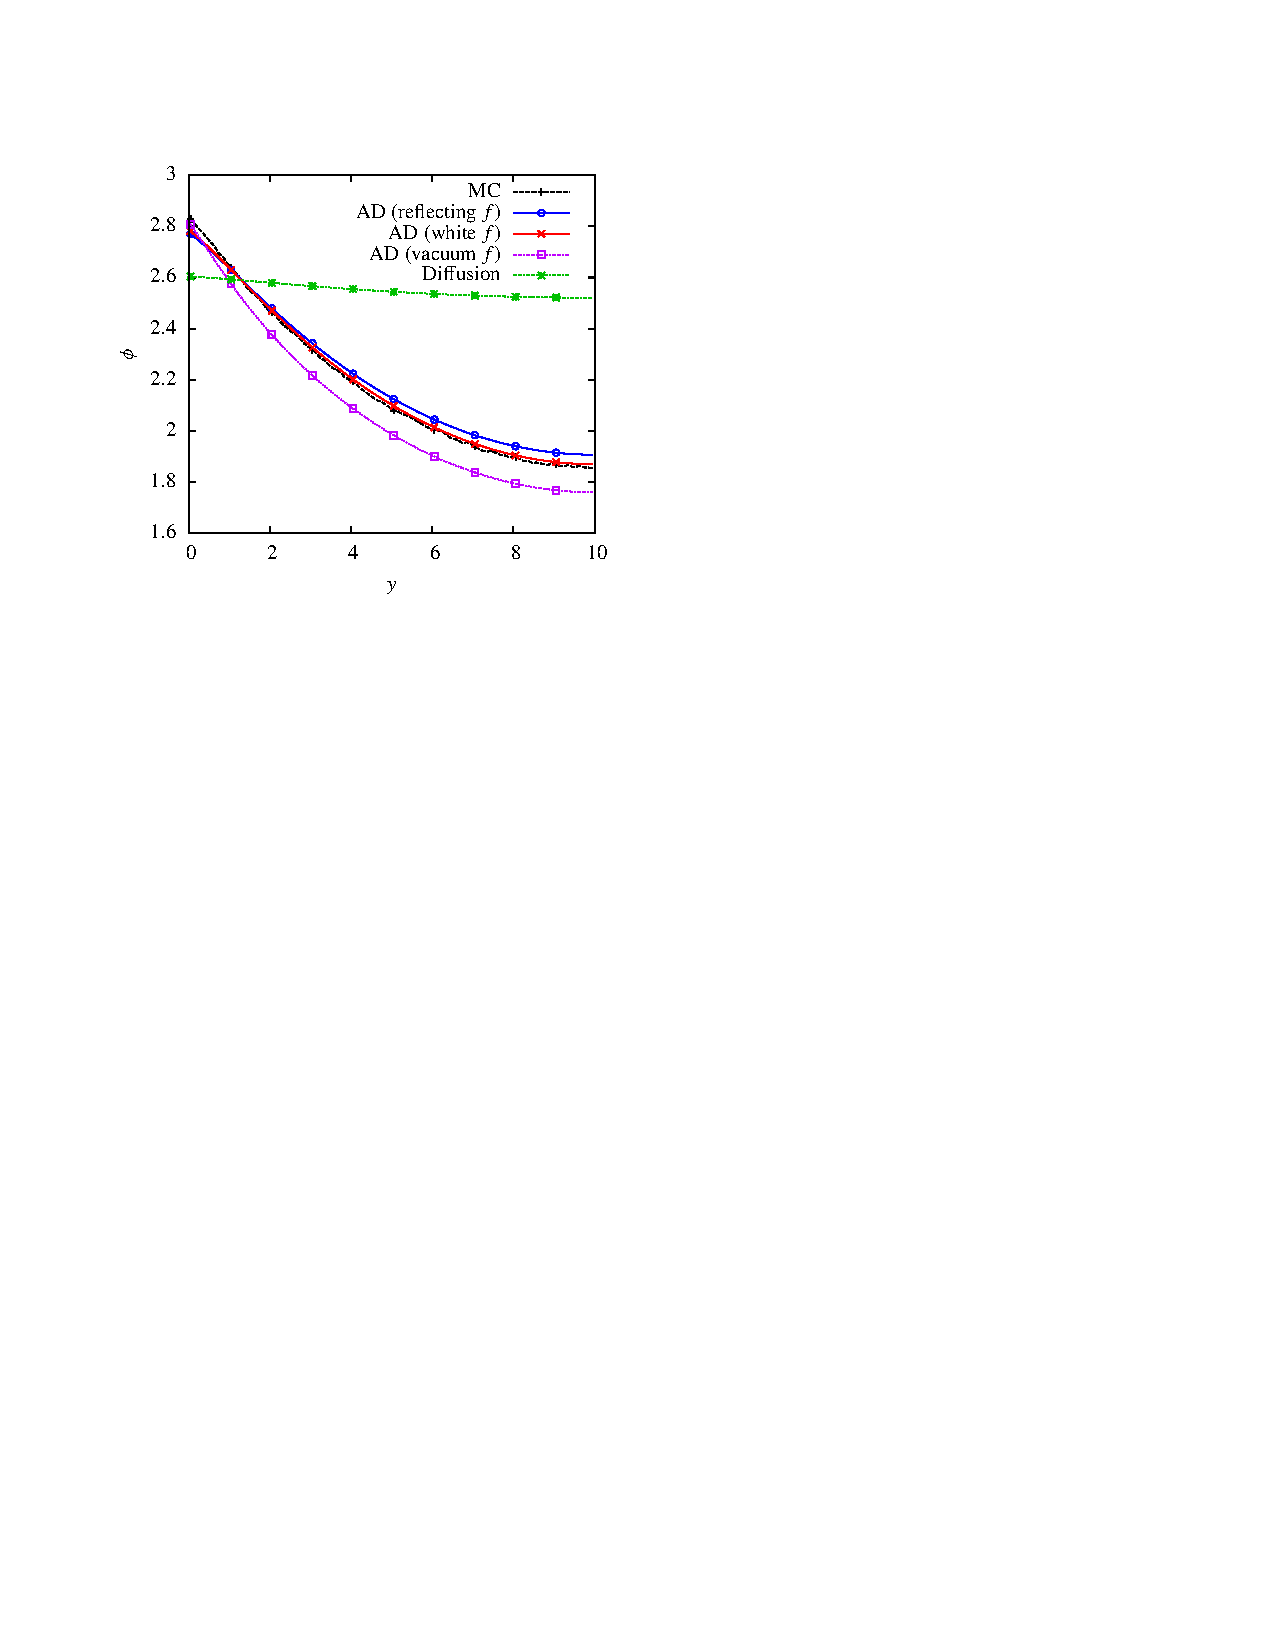
\includegraphics{example_figure}
  \caption{Captions are flush with the left.}
  \label{fig:voltage}
\end{figure}

Later on, we can include a table, even one that spans two columns such as
Table~\ref{tab:widetable}.
%%%%%%%%%%%%%%%%%%%%%%%%%%%%%%%%%%%%%%%%
\begin{table*}[htb]
  \centering
  \caption{Example of a Really Wide Table that Might Not Normally Fit in the Document}
  \begin{tabular}{llllllllll}\toprule
      & $\phi_T(0)$      & $\phi_T(10)$      & $\phi_T(20)$      &
      $\phi_D(0)$      & $\phi_D(10)$      & $\phi_D(20)$      & $\rho$      &
      $\varepsilon$      & $N_\text{it}$
\\ \midrule
$c=0.999$  & 0.9038 & 20.63 & 31.24 & 0.9087 & 20.63 & 31.23 & 0.2192 & $10^{-7}$ & 15
\\
$c=0.990$  & 0.3675 & 13.04 & 24.7 & 0.3696 & 13.04 & 24.69 & 0.2184 & $10^{-7}$ & 15
\\
$c=0.900$  & 0.009909 & 4.776 & 17.64 & 0.009984 & 4.786 & 17.63 & 0.2118 & $10^{-7}$ & 14
\\
$c=0.500$  & $6.069\times 10^{-5}$ & 2.212 & 15.53 & 6.213$\times 10^{-5}$ & 2.239 & 15.53 & 0.2068 & $10^{-7}$ & 13
\\
\bottomrule
\end{tabular}
  \label{tab:widetable}
\end{table*}
%%%%%%%%%%%%%%%%%%%%%%%%%%%%%%%%%%%%%%%%
Notice how the table reference uses a Roman numeral
for its numbering scheme, whereas the figure reference uses an Arabic numeral.
For one-column tables, use the \verb|table| environment; two-column tables use
\verb|table*|. The same applies to figures.

%%%%%%%%%%%%%%%%%%%%%%%%%%%%%%%%%%%%%%%%%%%%%%%%%%%%%%%%%%%%%%%%%%%%%%%%%%%%%%%%
\subsection{Another Subsection (Heading B)}
Excessive sectioning in a three-page document is discouraged, but here are more
subsections to demonstrate compliance with the ANS formatting guidelines.

\subsubsection{Susubsection Heading (Heading C)}
This subsubsection shows compliance with the ANS-specified standard. This level
of heading should be used rarely.

\subsubsection{Another Such Heading (Heading C)}
And, if you really think you need a third-level heading, you should make sure
that your subsection needs at least two of them.

%%%%%%%%%%%%%%%%%%%%%%%%%%%%%%%%%%%%%%%%%%%%%%%%%%%%%%%%%%%%%%%%%%%%%%%%%%%%%%%%
\section{Conclusions (Heading A)}

The included ANS style file and this clear example file are a panacea for
the hours of headache that invariably results from formatting a document in
Microsoft Word.

%%%%%%%%%%%%%%%%%%%%%%%%%%%%%%%%%%%%%%%%%%%%%%%%%%%%%%%%%%%%%%%%%%%%%%%%%%%%%%%%
\appendix
\section{Appendix}

Numbering in the appendix is different:
\begin{equation} \label{eq:appendix}
  2 + 2 = 5\,.
\end{equation}
and another equation:
\begin{equation} \label{eq:appendix2}
  a + b = c\,.
\end{equation}

%%%%%%%%%%%%%%%%%%%%%%%%%%%%%%%%%%%%%%%%%%%%%%%%%%%%%%%%%%%%%%%%%%%%%%%%%%%%%%%%
\section{Acknowledgments}
This material is based upon work supported by a Department of Energy Nuclear
Energy University Programs Graduate Fellowship.

%%%%%%%%%%%%%%%%%%%%%%%%%%%%%%%%%%%%%%%%%%%%%%%%%%%%%%%%%%%%%%%%%%%%%%%%%%%%%%%%
\bibliographystyle{ans}
\bibliography{bibliography}
\end{document}

